% ****** Start of file apssamp.tex ******
%
%   This file is part of the APS files in the REVTeX 4 distribution.
%   Version 4.0 of REVTeX, August 2001
%
%   Copyright (c) 2001 The American Physical Society.
%
%   See the REVTeX 4 README file for restrictions and more information.
%
% TeX'ing this file requires that you have AMS-LaTeX 2.0 installed
% as well as the rest of the prerequisites for REVTeX 4.0
%
% See the REVTeX 4 README file
% It also requires running BibTeX. The commands are as follows:
%
%  1)  latex apssamp.tex
%  2)  bibtex prb
%  3)  latex apssamp.tex
%  4)  latex apssamp.tex
%
%\documentclass[aps,prb,preprint,groupedaddress,showpacs]{revtex4-1}
\documentclass[aps,prl,preprint,superscriptaddress]{revtex4}
%\documentclass[aps,prl,twocolumn,superscriptaddress]{revtex4}
%\documentclass[aps,prl,twocolumn,superscriptaddress]{revtex4}
%\documentclass[aps,prb,twocolumn,groupedaddress]{revtex4-1}


%\documentclass[twocolumn,showpacs,preprintnumbers,amsmath,amssymb]{revtex4}
%\documentclass[preprint,showpacs,preprintnumbers,amsmath,amssymb]{revtex4}

% Some other (several out of many) possibilities
%\documentclass[preprint,aps]{revtex4}
%\documentclass[preprint,aps,draft]{revtex4}
%\documentclass[prb]{revtex4}% Physical Review B

\usepackage{graphics}
\usepackage{graphicx}% Include figure files
\usepackage{epstopdf}
\usepackage{dcolumn}% Align table columns on decimal point
\usepackage{bm}% bold math
\usepackage{amsmath}
\usepackage{amssymb}
\usepackage{latexsym}
\usepackage{epsfig}
\usepackage{amsbsy}
\usepackage{array}
\usepackage{amssymb}
\usepackage{setspace}
\usepackage{bm}
\usepackage{float}
\usepackage[caption = false]{subfig}

\newcommand{\ssint}{ - \!\!\!\!\! \int }
\def\sint{\ifmmode{- \!\!\!\!\!\! \int}
    \else{\hbox{$- \!\!\!\! \int \ $}}\fi}


\newcommand{\bsigma}{\boldsymbol{\sigma}}
\newcommand{\bmu}{\boldsymbol{\mu}}
\newcommand{\bvepsilon}{\boldsymbol{\varepsilon}}
\newcommand{\bepsilon}{\boldsymbol{\epsilon}}
\newcommand{\balpha}{\boldsymbol{\alpha}}
\newcommand{\bkappa}{\boldsymbol{\kappa}}
\newcommand{\bchi}{\boldsymbol{\chi}}
\newcommand{\bgamma}{\boldsymbol{\gamma}}
\newcommand{\bpsi}{\boldsymbol{\psi}}
\newcommand{\bnu}{\boldsymbol{\nu}}
\newcommand{\bzero}{\boldsymbol{0}}
\newcommand{\bbeta}{\boldsymbol{\beta}}
\newcommand{\bSigma}{\boldsymbol{\Sigma}}

\newcommand{\va}{\varphi}
\newcommand{\ep}{\epsilon}
\newcommand{\mbf}{{\bf m}}
\newcommand{\pbf}{{\bf p}}
\newcommand{\xbf}{{\bf x}}
\newcommand{\weak}{\rightharpoonup}
\newcommand{\rgoto}{\rightarrow}

\newcommand{\grad}{\mbox{grad}}
\newcommand{\curl}{\mbox{curl}}
\newcommand{\dive}{\mbox{div}}


\newcommand{\tr}{\mbox{tr}}

\newcommand{\ba}{\mathbf{a}}
\newcommand{\bb}{\mathbf{b}}
\newcommand{\bc}{\mathbf{c}}
\newcommand{\bd}{\mathbf{d}}
\newcommand{\be}{\mathbf{e}}
\newcommand{\bsf}{\mathbf{f}}
\newcommand{\bg}{\mathbf{g}}
\newcommand{\bsi}{\mathbf{i}}
\newcommand{\bk}{\mathbf{k}}
\newcommand{\bn}{\mathbf{n}}
\newcommand{\bo}{\mathbf{o}}
\newcommand{\bp}{\mathbf{p}}
\newcommand{\bq}{\mathbf{q}}
\newcommand{\br}{\mathbf{r}}
\newcommand{\bs}{\mathbf{s}}
\newcommand{\bt}{\mathbf{t}}
\newcommand{\bu}{\mathbf{u}}
\newcommand{\bv}{\mathbf{v}}
\newcommand{\bw}{\mathbf{w}}
\newcommand{\bx}{\mathbf{x}}
\newcommand{\by}{\mathbf{y}}
\newcommand{\bz}{\mathbf{z}}

\newcommand{\bca}{\mathbf{A}}
\newcommand{\bcb}{\mathbf{B}}
\newcommand{\bcc}{\mathbf{C}}
\newcommand{\bcd}{\mathbf{D}}
\newcommand{\bce}{\mathbf{E}}
\newcommand{\bcf}{\mathbf{F}}
\newcommand{\bcg}{\mathbf{G}}
\newcommand{\bch}{\mathbf{H}}
\newcommand{\bck}{\mathbf{K}}
\newcommand{\bcj}{\mathbf{J}}
\newcommand{\bci}{\mathbf{I}}
\newcommand{\bcl}{\mathbf{L}}
\newcommand{\bcm}{\mathbf{M}}
\newcommand{\bcn}{\mathbf{N}}
\newcommand{\bco}{\mathbf{O}}
\newcommand{\bcp}{\mathbf{P}}
\newcommand{\bcq}{\mathbf{Q}}
\newcommand{\bcr}{\mathbf{R}}
\newcommand{\bcs}{\mathbf{S}}
\newcommand{\bct}{\mathbf{T}}
\newcommand{\bcu}{\mathbf{U}}
\newcommand{\bcv}{\mathbf{V}}
\newcommand{\bcw}{\mathbf{W}}
\newcommand{\bcx}{\mathbf{X}}
\newcommand{\bcz}{\mathbf{Z}}
\newcommand{\bcy}{\mathbf{Y}}

\usepackage{hyperref}
\hypersetup{
    colorlinks=true,
    linkcolor=blue,
    filecolor=magenta,      
    urlcolor=cyan,
}

%\nofiles

\begin{document}
	
	
	\title{Predator-Prey Model}% Force line breaks with \\
	
	\author{Connor Hann, Xiaomeng Jia, Peifan Liu and Xinyu Wu}
	\affiliation{Physics Department, Duke University}
	
	
	\date{\today}
	
	\begin{abstract}
	In this article, a classical predator-prey model is numerically explored upon several given rules. By moving a random number of sharks and fish on a 2D torus lattice and imitating the real-world rules that fish swim and breed offspring, sharks hunt fish, breed and starve to death for a given time, we dynamically show the revolution of populations of fish and sharks. It is shown that given proper initial conditions, they experience stable periodic solutions which look similar to the solutions of the Lotka-Volterra Model. For this simulation, however, a modified Lotka-Volterra Model is used due to the limited capacity of the lattice to describe the dynamics of these two species. (Github link: \href{https://github.com/xiaoao-duke/Group-Project-2.git}{https://github.com/xiaoao-duke/Group-Project-2.git} )
	\end{abstract}
	
	\maketitle
	
	
	
	\section{Background} 
Modeling the interactions between predator and prey is a question of great ecological importance, as accurate models can allow one to make reliable predictions and thereby inform decisions in conservation, habitat preservation, hunting regulations, etc. 
\section{Classical Lotka-Volterra Model}	
There exist a variety of methods for modeling the interactions between predator and prey, and these models, though simple, are often in quite good agreement with what is observed. Take the classic Lotka-Volterra Model as an example. While this model is nothing more than a set of first-order nonlinear differential equations that one may solve numerically for a particular set of initial conditions, the model is capable of providing a qualitatively accurate description of the data, as is shown in Fig.~\ref{LV}. 

\begin{figure}[H]
	\centering
	\subfloat{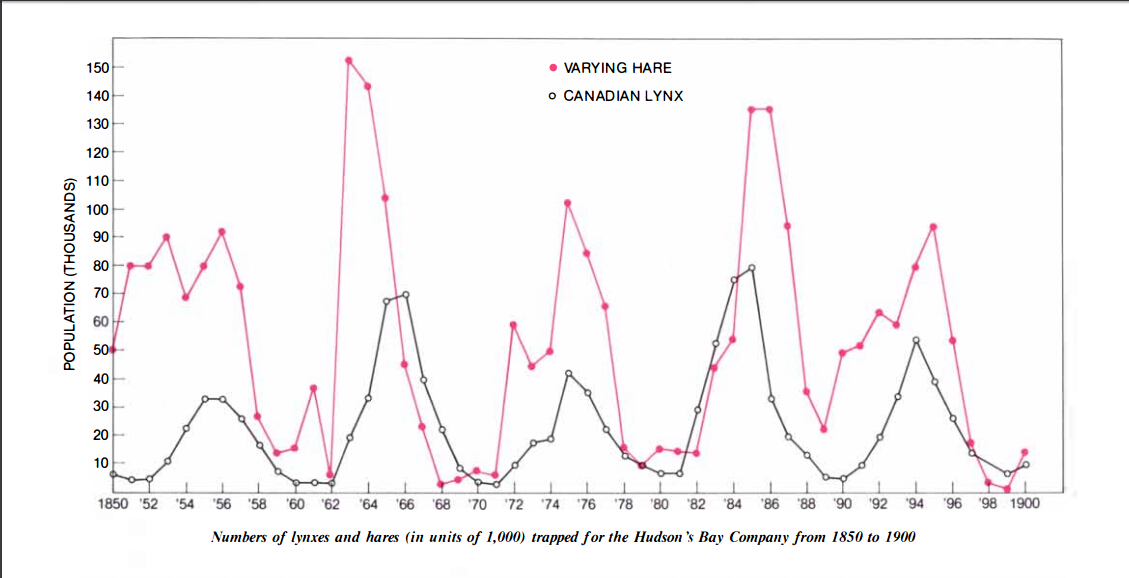
\includegraphics[width = 0.7\textwidth]{LV_data}}\\
	\subfloat{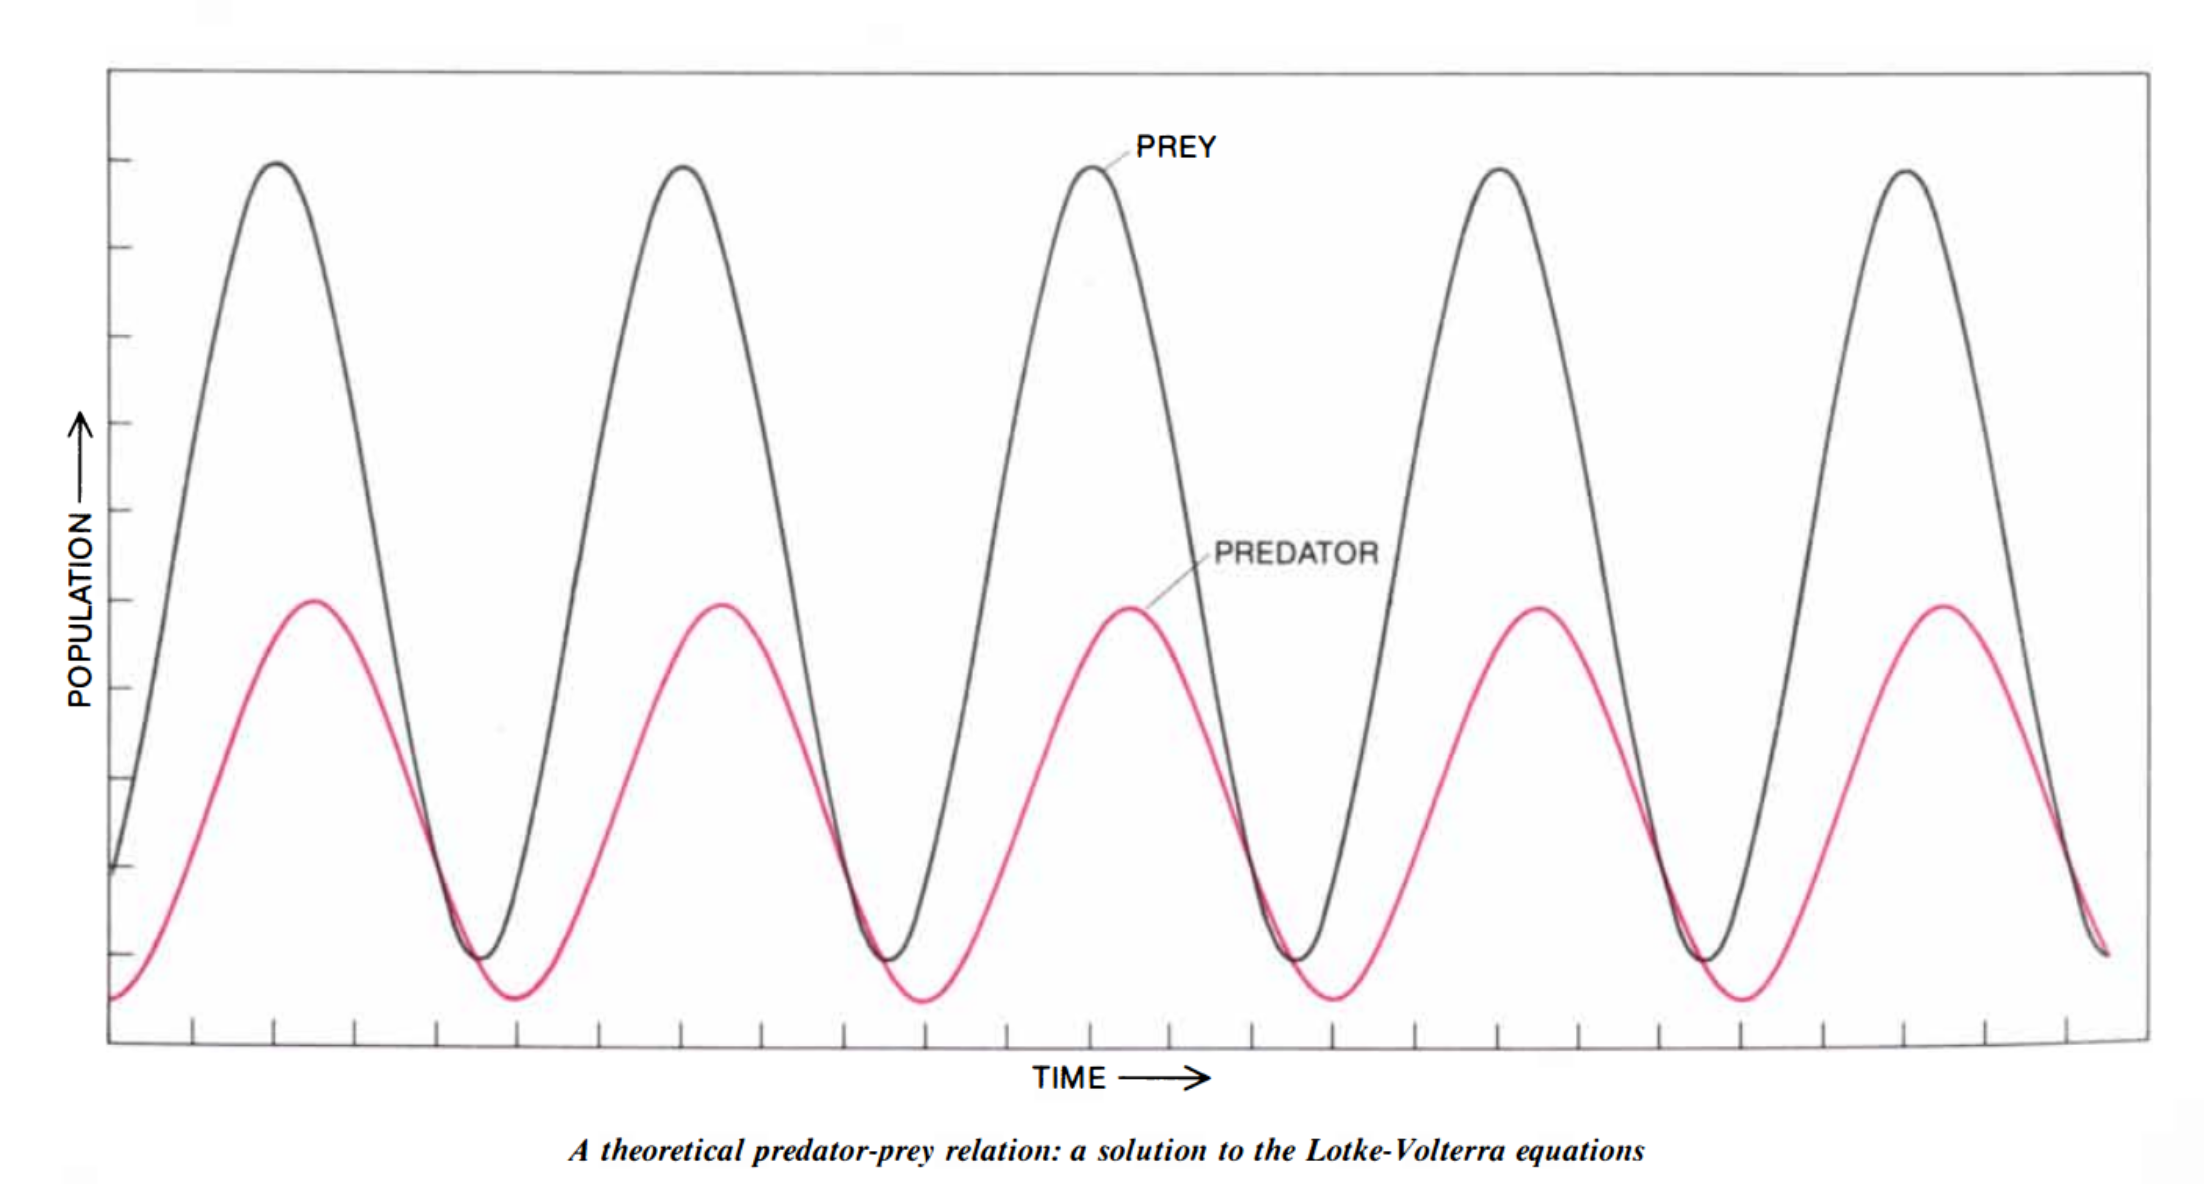
\includegraphics[width = 0.7\textwidth]{LV_prediction}}
	\caption{(Top) experimental data of Hare and Lynx populations, (Bottom) predictions from the Lotka-Volterra equations. }
	\label{LV} 
\end{figure}

In this work we study the behavior of a slightly different model, one that  is similar to the Lotka-Volterra Model in that it consists of only a simple set of rules, but the nature of the actual simulation is quite different. In our case, we consider two populations, sharks and fish living on a two-dimensional lattice. We simulate the movement and behavior of each shark and fish individually and can observe fluctuations of the two populations as a function of time. Unlike the Lotka-Volterra Model, however, we are able to see exactly where all of the sharks and fish are and this allows us to attain a deeper understanding of what causes the fluctuations in populations and the conditions that may lead to extinction. The classical Lotka-Volterra Model is given by:


\begin{equation}
x' = x(\alpha-\beta y)
\end{equation}
\begin{equation}
y' = -y(\gamma -\delta x)
\end{equation}

where $\alpha x$ is the growth term which leads to exponential growth of prey population in absence of predators; $-\beta yx$ is the loss term which depends both on numbers of predators $y$ and number of prey $x$; $-\gamma y$ is the exponential decay term for predators; $\delta xy$ is the gain term for predators which depends on populations of both species. The Lotka-Volterra Model has periodic solutions where peaks of predator population shifts $\pi/2$ with respect to the prey population.

\section{Implementation}

The model we consider is remarkably simple in that there are only five user input parameters: the initial number of sharks $n0\_sharks$, initial number of fish $n0\_fish$, the time it takes fish to breed $breed\_age\_Fish$, the time it takes sharks to breed $breed\_age\_Shark$, and the time it takes a shark to starve to death $starve\_time$. To begin the simulation, one creates $n0\_sharks$ sharks and $n0\_fish$ fish at random locations on a two-dimensional lattice, and each fish or shark is given a random age between $breed\_age\_Fish$ and $breed\_age\_Shark$, respectively. At each subsequent time step of the simulation both sharks and fish will swim around the grid, and the sharks will attempt to eat the fish. Below we discuss the specific rules that dictate the movements of the fish and sharks.

\subsection{Fish Movement}
During a time step, each fish looks at the four adjacent lattice sites and randomly chooses an empty site to which to move. If no lattice sites are available, the fish remains in its current position. We implement periodic boundary conditions so that if a fish moves through one boundary it reappears on the boundary on the opposite side, i.e. our two-dimensional grid is actually a topological torus. The age of the fish is increased by one in each time step, regardless it moves or not. If the age of the fish reaches $breed\_age\_Fish$, an additional fish is created at the site the fish has just moved from, and the ages of both fish are set to 0.

\subsection{Shark Movement}
The goal of the sharks is to eat fish, so during a time step each shark will look for fish on the adjacent lattice sites. If fish are found, the shark chooses one randomly and moves to the fish's position on the lattice, deleting and ``eating'' the fish. If no fish are available the sharks move just like the fish, choosing an available lattice site to move to randomly. Like the fish, the age of the sharks is increased by one each time step, and sharks breed in the same way as the fish once they have reached $breed\_age\_Shark$. Unlike the fish, however, the sharks will starve if they do not find food. An array keeps track of how long it has been since each shark has last eaten a fish, and if a shark has not found a fish within $starve\_time$ time steps, it ``starves'' to death and is deleted from the simulation.

\subsection{Program Structure}
We use a set of five arrays to keep track of the information necessary to run the simulation as described above. Two $N \times N$ arrays, $Sharks$ and $Fish$, are used to keep track of the positions of the sharks and fish respectively. If the $(i,j)$ site is empty the arrays hold the value $-1$, otherwise the site holds the age of the shark or fish. Two additional arrays $Sharkmove$ and $Fishmove$ are used to store the new positions of the sharks and fish as an update is being performed, allowing us to ensure that each shark or fish is moved only once and that two animals are not moved onto the same lattice site. Finally, a fifth array $Sharkstarve$ stores the amount of time since each shark has last eaten. The arrays are updated, first fish then sharks, via the rules above. One can plot the positions of the sharks and fish at any time step, and an example plot is shown in Fig.~\ref{ex}.

\begin{figure}[H]
	\centering
	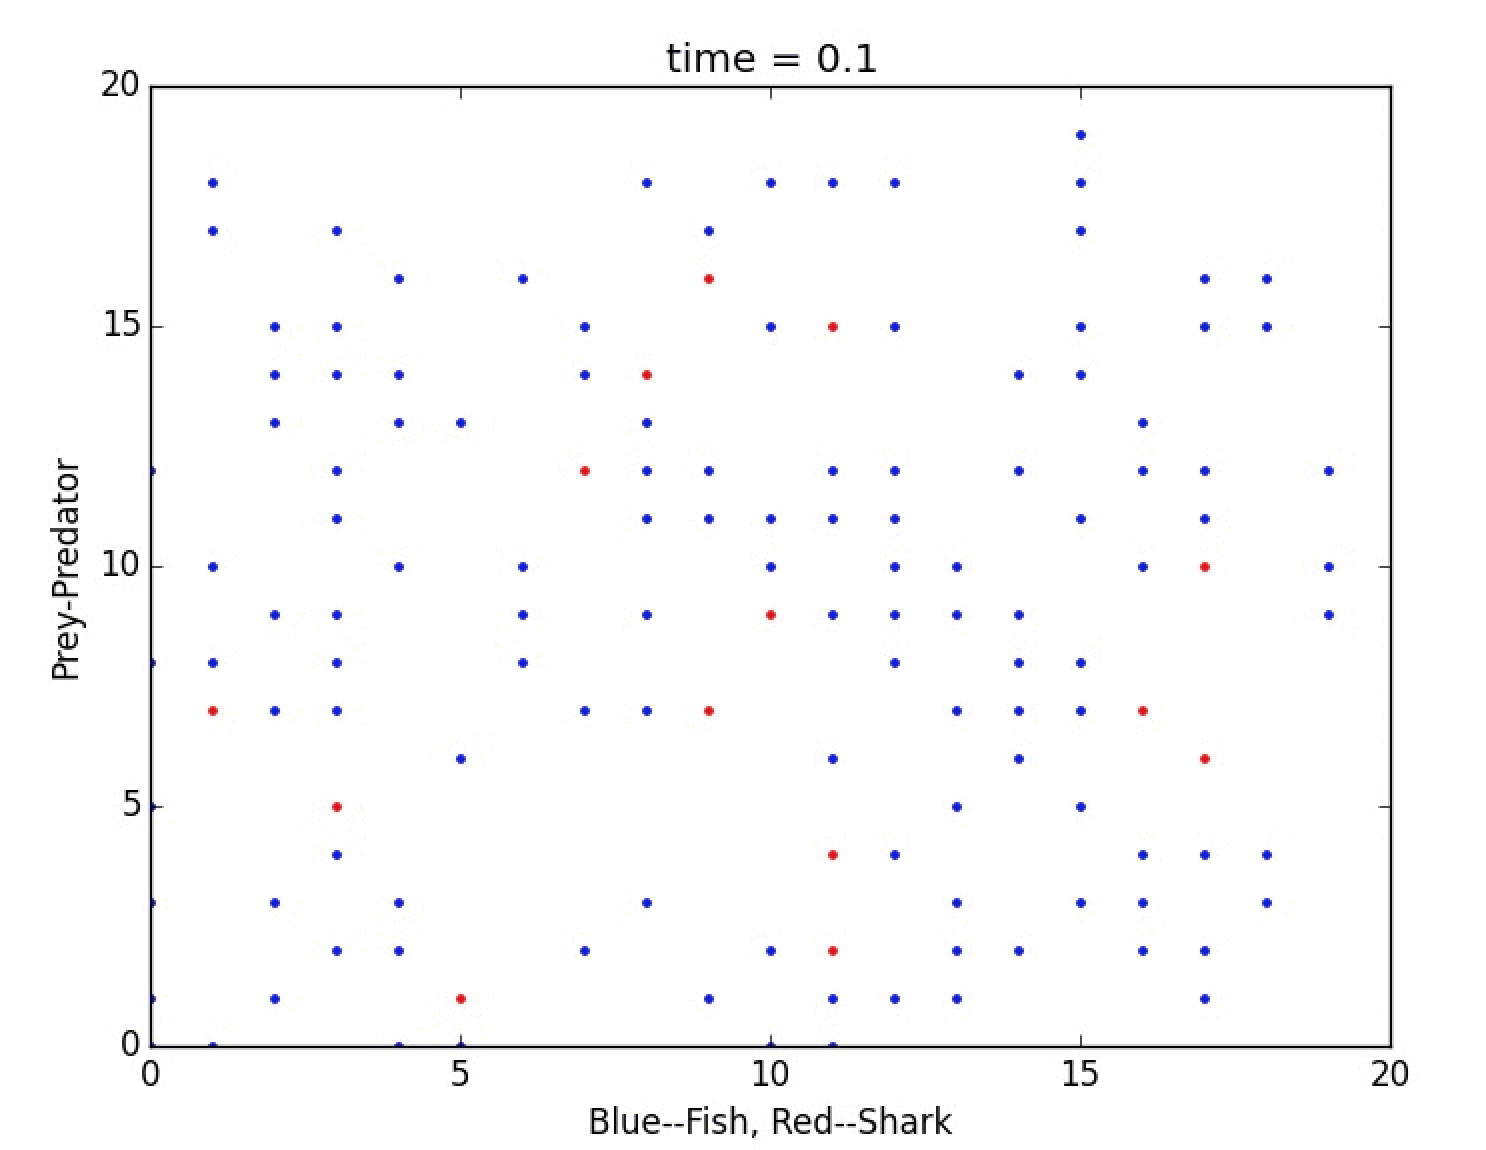
\includegraphics[width = 0.7\textwidth]{example}
	\caption{A typical configuration of sharks and fish on a $20 \times 20$ lattice}
	\label{ex} 
\end{figure}


\section{Numerical Results}

By choosing a $100*100$ 2D torus grid where 2000 fish and 200 sharks of random ages are randomly put as initial condition, it can be seen that as time goes on, the populations of fish and shark experience periodic variations. The number of fish increases most significantly when number of sharks reaches a valley, and decreases most sharply when shark reaches its peaks, as shown in Fig.3. The phase plane is shown in Fig.4. If we trace the dynamics of the system in each time step, it can be seen that sometimes fish fill out the whole grid and sometimes become almost extinct (Fig.6-9). This reminds us that the capacity of the grid is the upper constraint for the fish number, so the classical Lotka-Volterra equations must be modified to adapt to this simulation. Instead of exponential growth, the fish number should be described as logistic, and so does the sharks:

\begin{equation}
x' = x(A - Bx - Cy)
\end{equation}
\begin{equation}
y' = -y(D - EY -Fx)
\end{equation}
which gives the analytic phase diagram (Fig.5) that properly coincide with simulation result (Fig.4).

\begin{figure}[H]
	\centering
	\subfloat{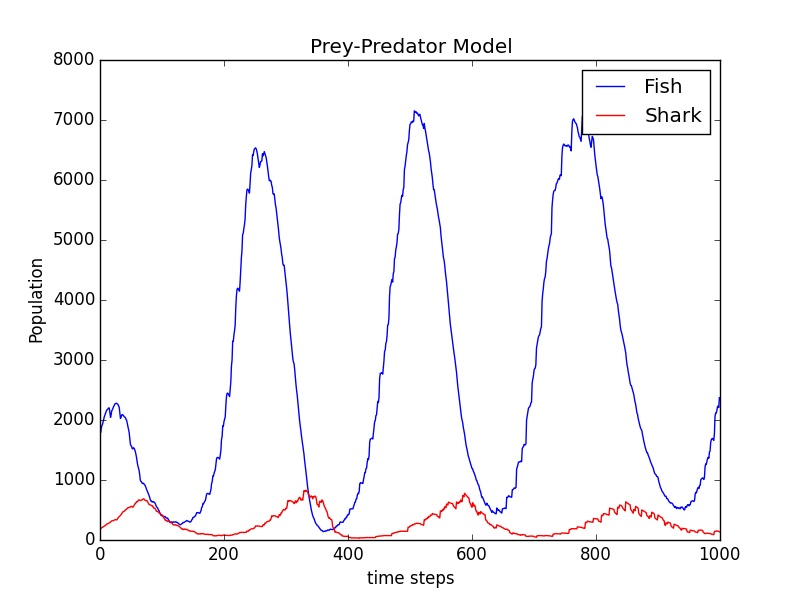
\includegraphics[width = 0.65\textwidth]{pop3.jpg}}
	\caption{Population evolution of fish and sharks.}
	\label{more_clusters} 
\end{figure}


\begin{figure}[H]
	\centering
	\subfloat{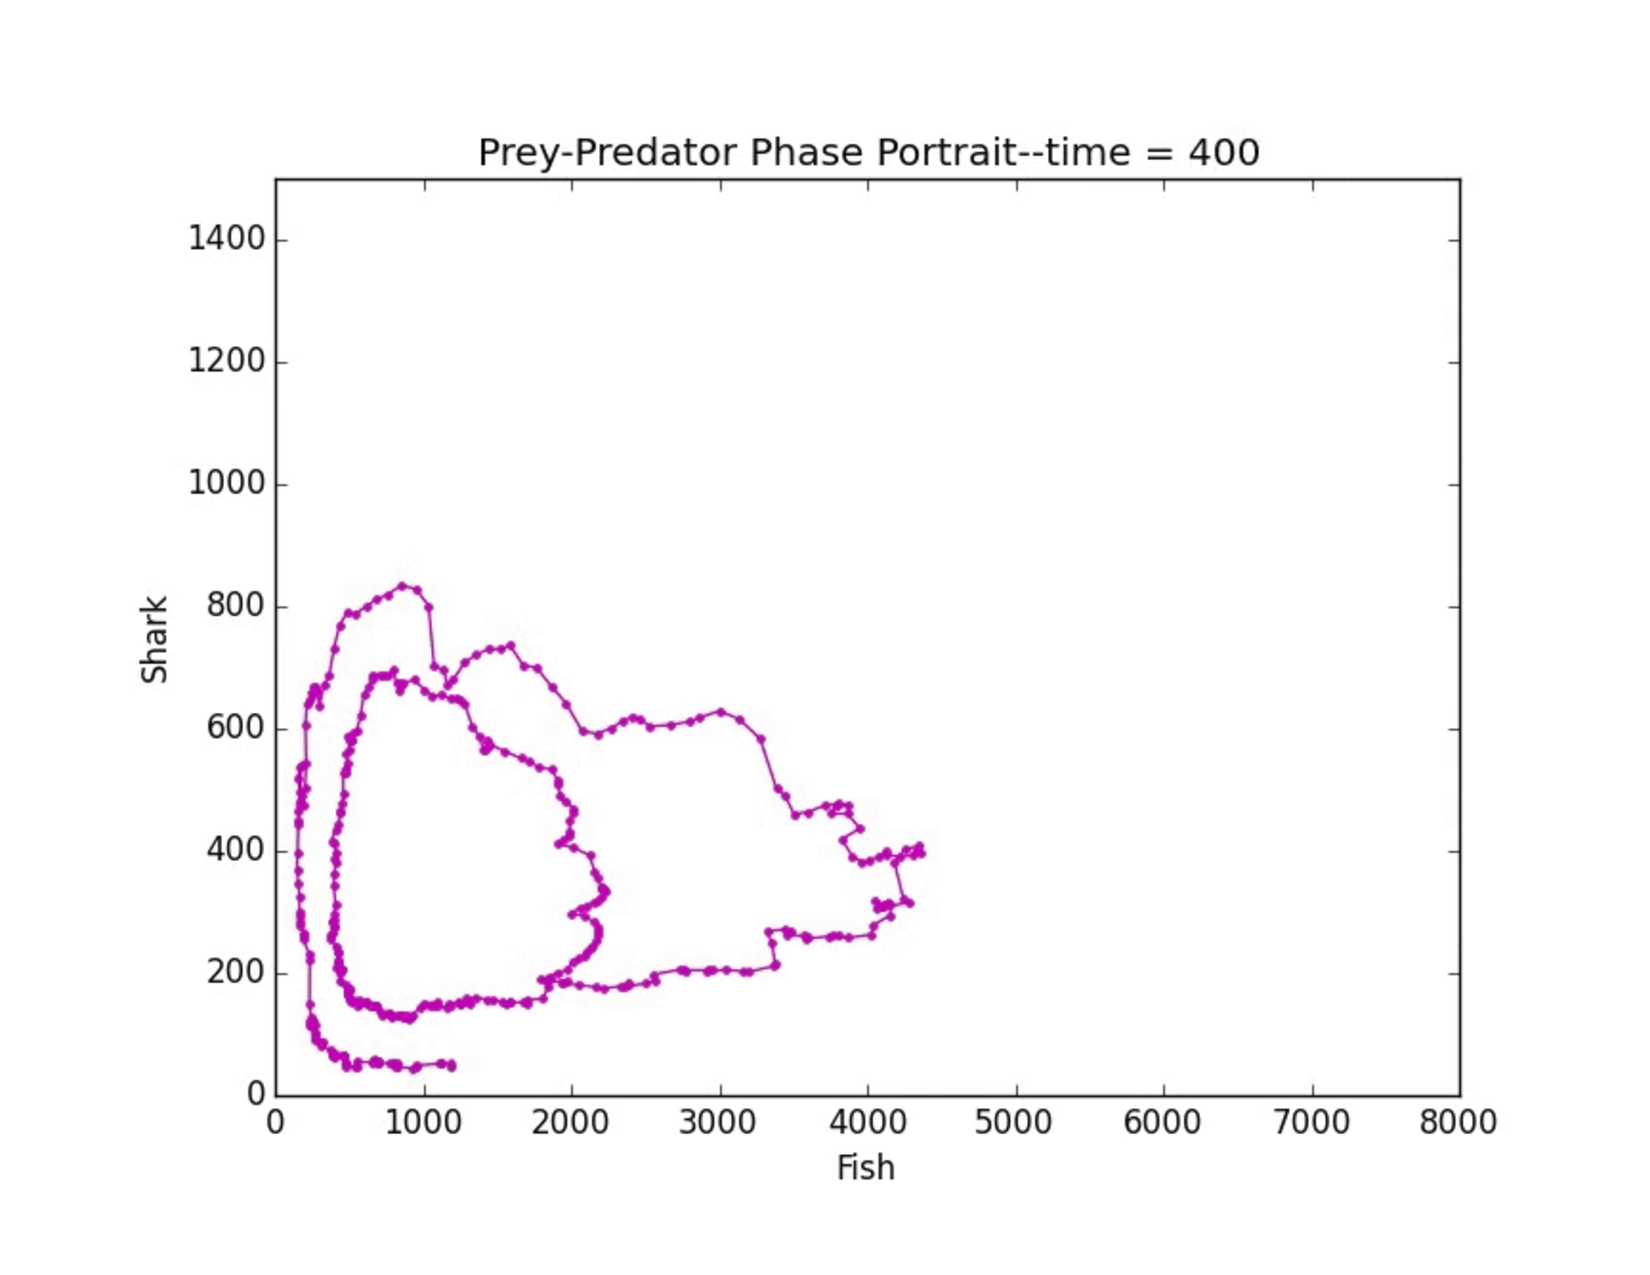
\includegraphics[width = 0.75\textwidth]{phase_portrait.pdf}}	
	\caption{Population evolution of fish and sharks in phase space.}
	\label{more_clusters} 
\end{figure}

\begin{figure}[H]
	\centering
	\subfloat{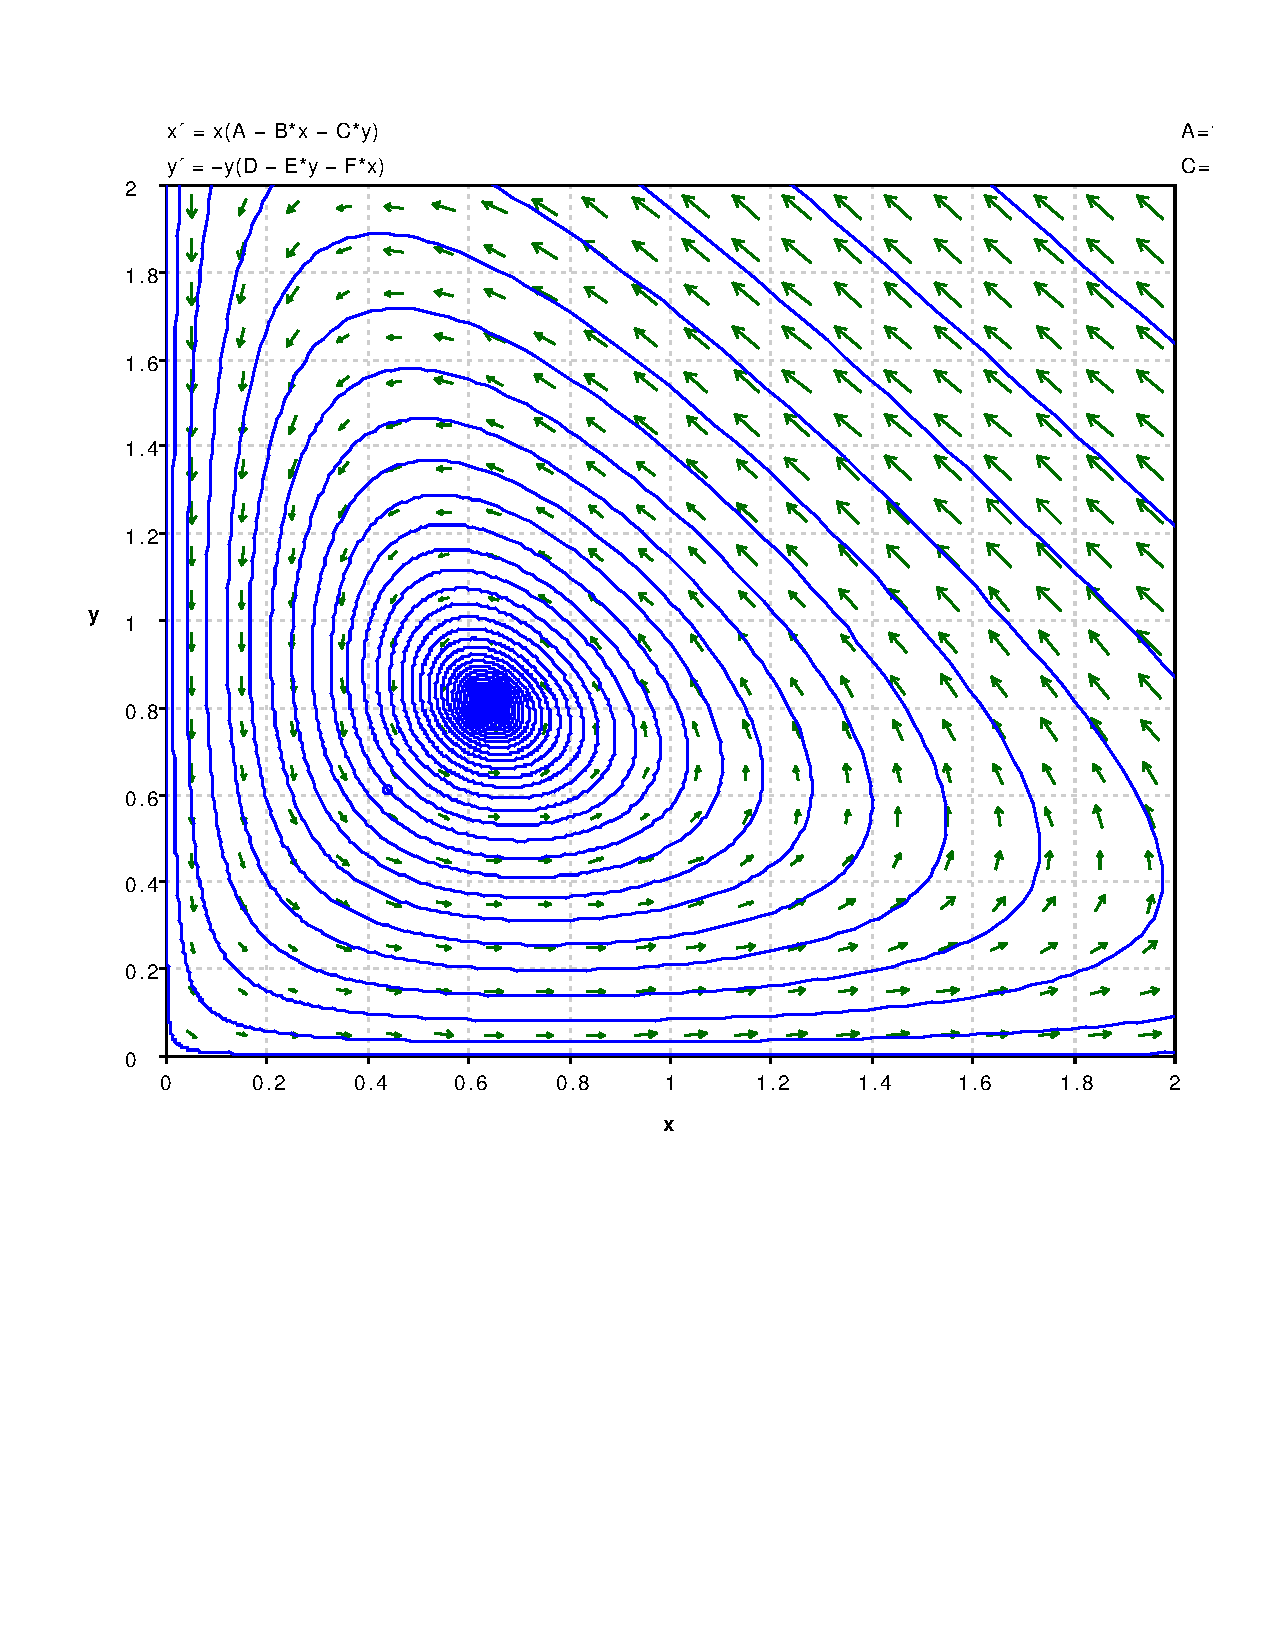
\includegraphics[width = 0.7\textwidth]{PreyPredator.pdf}}
	\caption{Phase diagram of modified Lotka-Volterra equations.}
	\label{more_clusters} 
\end{figure}

\begin{figure}[H]
	\centering
	\subfloat{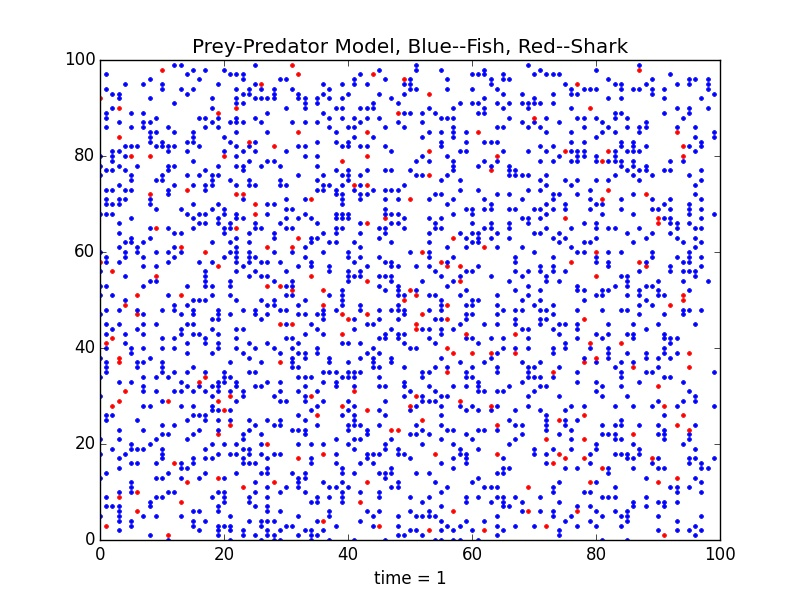
\includegraphics[width = 0.33\textwidth]{1.jpg}}
	\subfloat{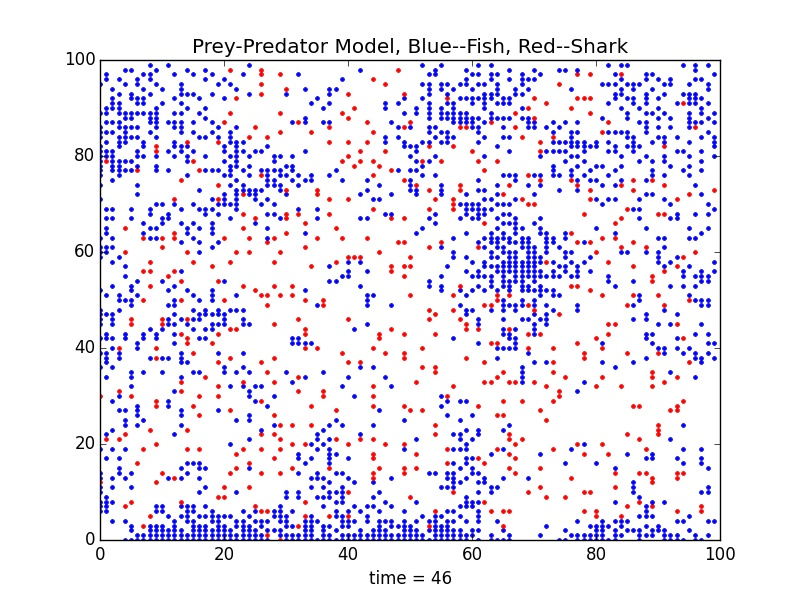
\includegraphics[width = 0.33\textwidth]{46.jpg}}
	\subfloat{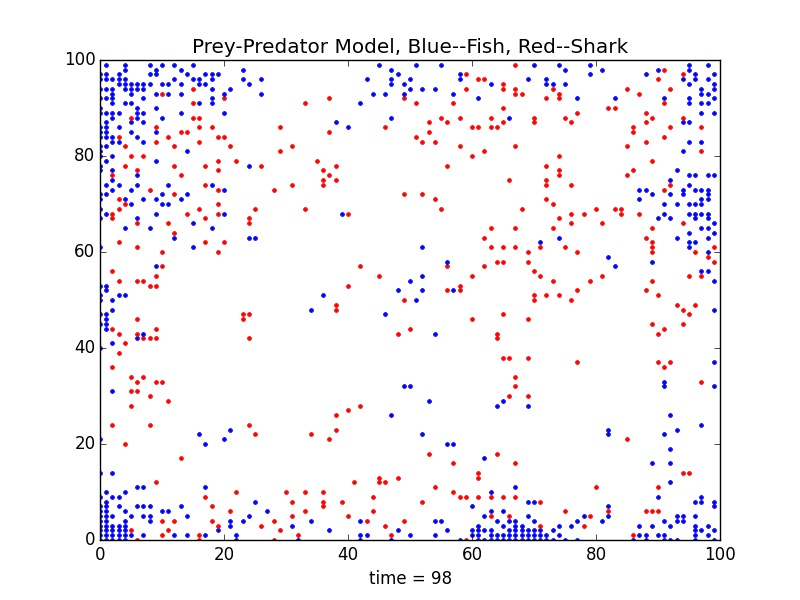
\includegraphics[width = 0.33\textwidth]{98.jpg}}	
	\caption{Population evolution of fish and sharks.}
	\label{more_clusters} 
\end{figure}

\begin{figure}[H]
	\centering
	\subfloat{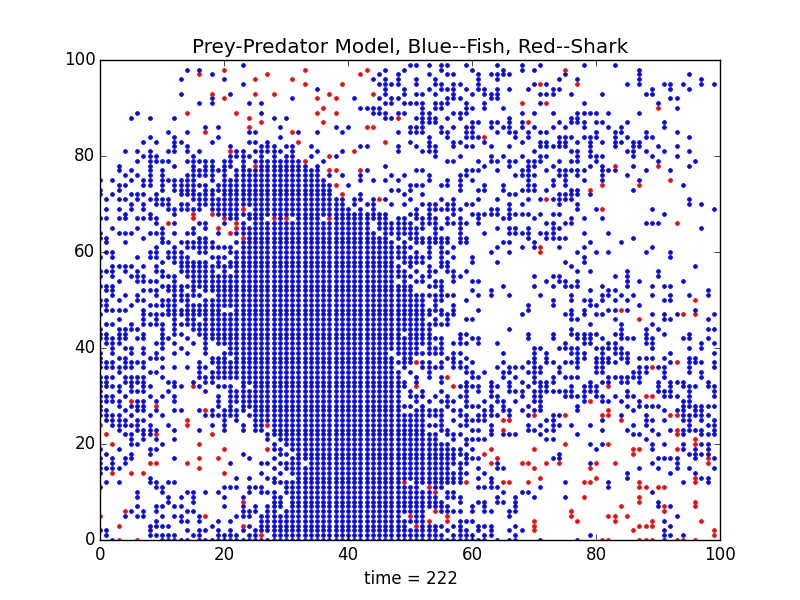
\includegraphics[width = 0.33\textwidth]{222.jpg}}
	\subfloat{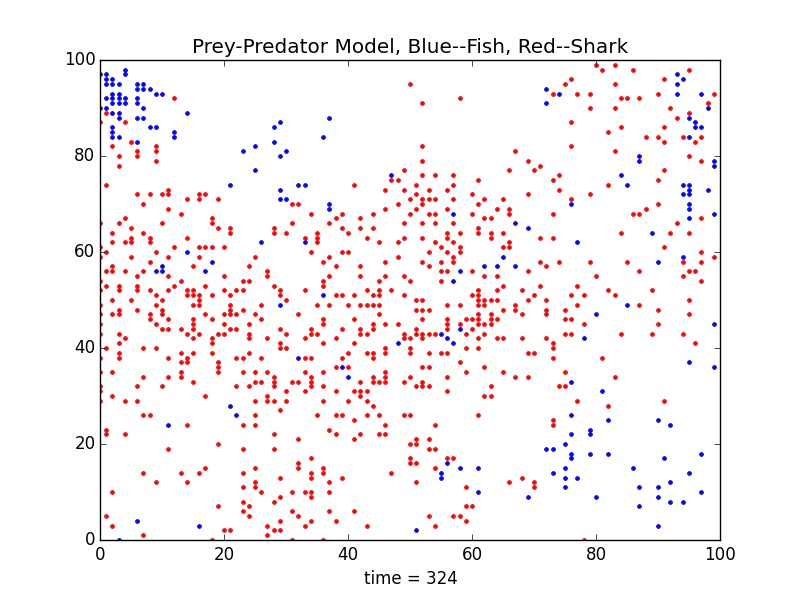
\includegraphics[width = 0.33\textwidth]{324.jpg}}
	\subfloat{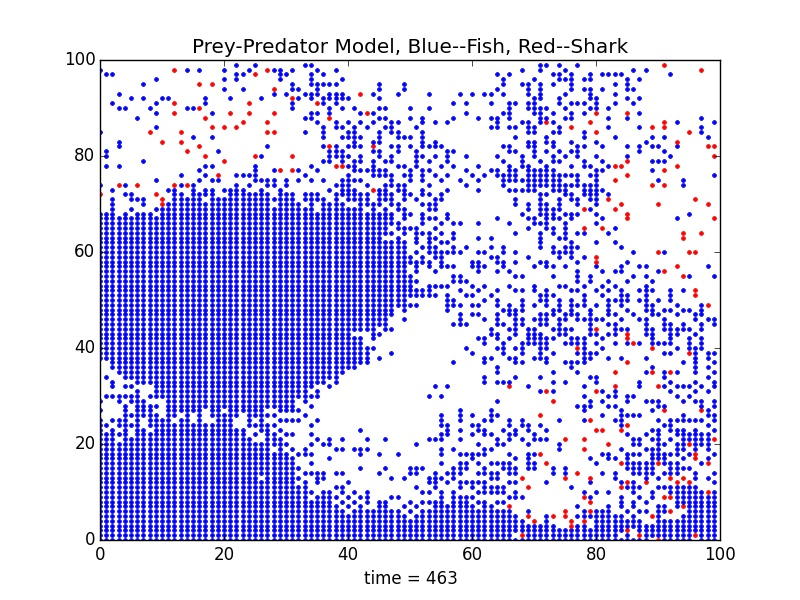
\includegraphics[width = 0.33\textwidth]{463.jpg}}
	\caption{Population evolution of fish and sharks.}
	\label{more_clusters} 
\end{figure}

This initial condition gives a stable periodic revolution. However, if initial conditions are far off the stable point, extinction of sharks or fish can be observed (Fig.8-9).


\begin{figure}[H]
	\centering
	\subfloat{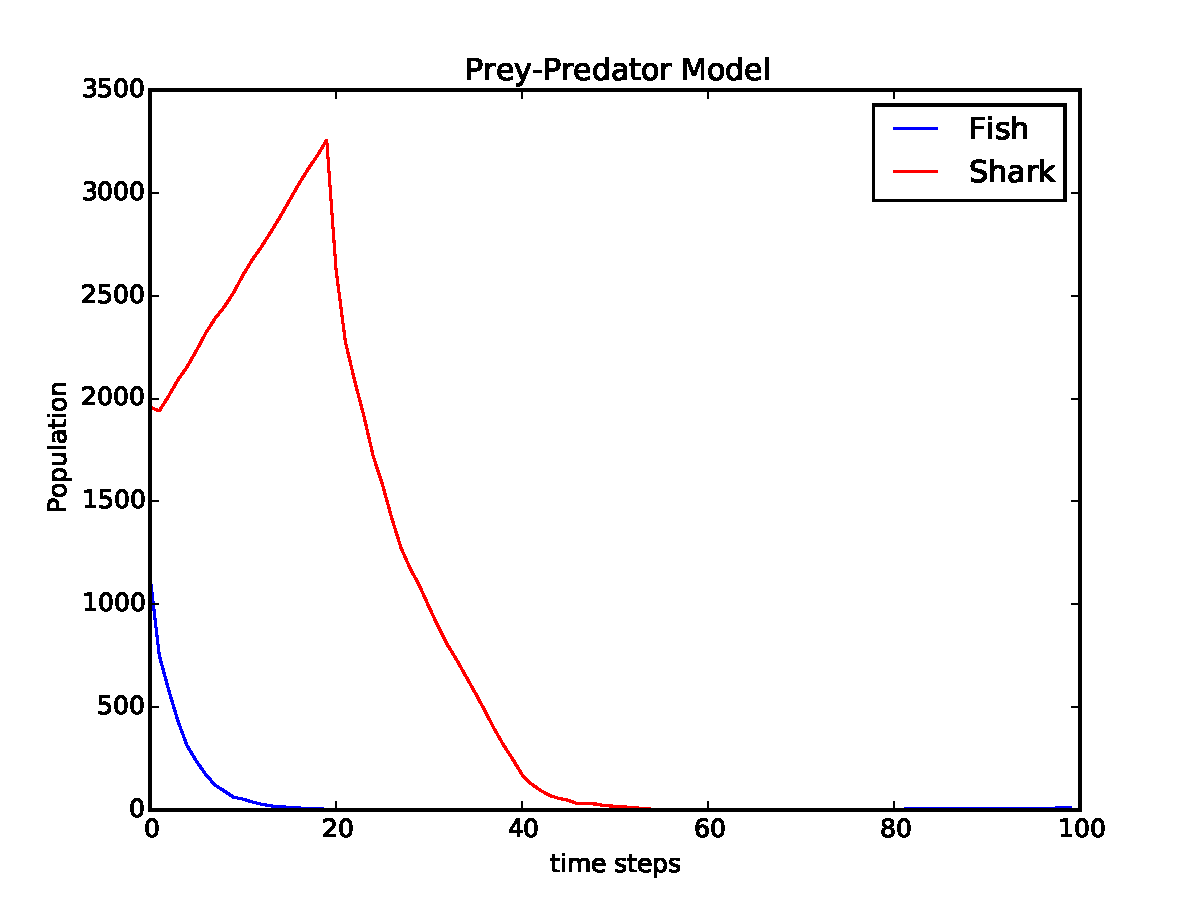
\includegraphics[width = 0.7\textwidth]{pop5.pdf}}
	\caption{Extinction of both fish and sharks.}
	\label{more_clusters} 
\end{figure}

\begin{figure}[H]
	\centering
	\subfloat{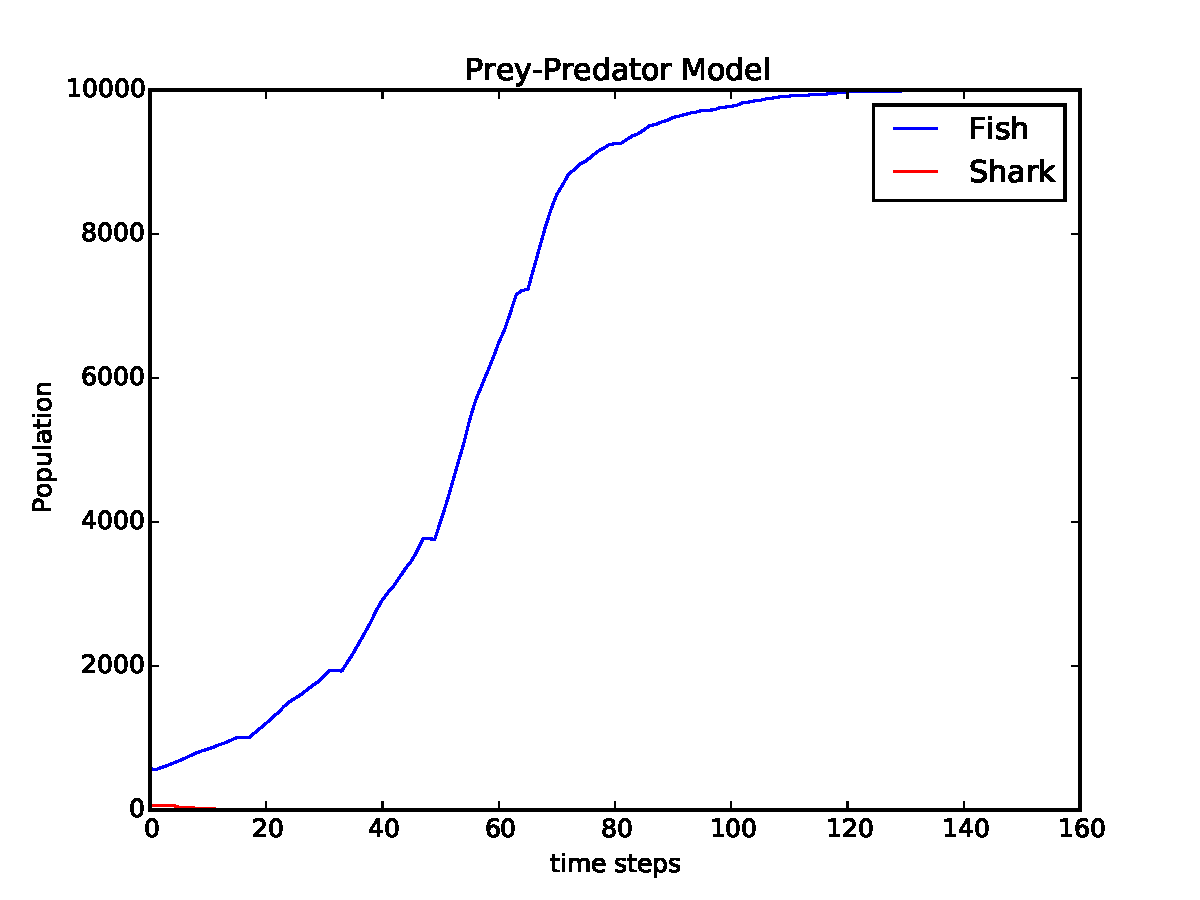
\includegraphics[width = 0.7\textwidth]{pop6.pdf}}
	\caption{Extinction of sharks.}
	\label{more_clusters} 
\end{figure}
 
\section{Conclusion}
The shark and fish predator-prey model we have described above possesses many qualities of the Lotkka-Voltera model, such as the ability of each species to go extinct ant the ability oscillate around an equilibrium. Indeed, we have show that the results of the simulation, when considered in phase space, are in good agreement with a modified version of the Lotkka-Voltera model. What distinguishes our model, however, is that we are able to observe the individual members of the species in real time, allowing us to gain a better intuition for why fluctuations in populations occur in the first place, and why certain initial conditions are liable to produce mass extinctions. 
  
\end{document}
	
	%
	% ****** End of file apssamp.tex ******
